
\begin{figure}[ht]
    \centering

\tikzset{every picture/.style={line width=0.75pt}} %set default line width to 0.75pt        

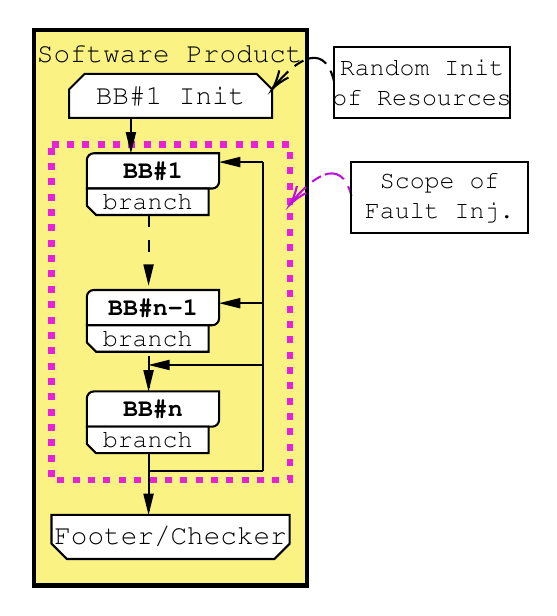
\begin{tikzpicture}[x=0.75pt,y=0.75pt,yscale=-0.85,xscale=0.85]
%uncomment if require: \path (0,385); %set diagram left start at 0, and has height of 385

%Shape: Rectangle [id:dp7802817346854477] 
\draw  [fill={rgb, 255:red, 248; green, 231; blue, 28 }  ,fill opacity=0.54 ][line width=1.5]  (375,25) -- (530,25) -- (530,340) -- (375,340) -- cycle ;
%Snip Same Side Corner Rect [id:dp4511869170411664] 
\draw  [fill={rgb, 255:red, 255; green, 255; blue, 255 }  ,fill opacity=1 ] (395,58.75) -- (403.75,50) -- (501.25,50) -- (510,58.75) -- (510,75) -- (510,75) -- (395,75) -- (395,75) -- cycle ;
%Rounded Diagonal Corner Rect [id:dp4147933552058153] 
\draw  [fill={rgb, 255:red, 255; green, 255; blue, 255 }  ,fill opacity=1 ] (405,99) .. controls (405,96.79) and (406.79,95) .. (409,95) -- (480,95) .. controls (480,95) and (480,95) .. (480,95) -- (480,111) .. controls (480,113.21) and (478.21,115) .. (476,115) -- (405,115) .. controls (405,115) and (405,115) .. (405,115) -- cycle ;
%Straight Lines [id:da5031724996809185] 
\draw  [dash pattern={on 4.5pt off 4.5pt}]  (440,130) -- (440,168) ;
\draw [shift={(440,170)}, rotate = 270] [fill={rgb, 255:red, 0; green, 0; blue, 0 }  ][line width=0.08]  [draw opacity=0] (12,-3) -- (0,0) -- (12,3) -- cycle    ;
%Shape: Rectangle [id:dp3861789631911239] 
\draw  [color={rgb, 255:red, 230; green, 33; blue, 215 }  ,draw opacity=1 ][dash pattern={on 2.53pt off 3.02pt}][line width=2.25]  (385,90) -- (520,90) -- (520,280) -- (385,280) -- cycle ;
%Snip Single Corner Rect [id:dp4150717653667523] 
\draw  [fill={rgb, 255:red, 255; green, 255; blue, 255 }  ,fill opacity=1 ] (474.01,130) -- (410.25,130) -- (405,124.75) -- (405,115) -- (474.01,115) -- cycle ;
%Rounded Diagonal Corner Rect [id:dp6179685400839223] 
\draw  [fill={rgb, 255:red, 255; green, 255; blue, 255 }  ,fill opacity=1 ] (405,176.5) .. controls (405,174.29) and (406.79,172.5) .. (409,172.5) -- (480,172.5) .. controls (480,172.5) and (480,172.5) .. (480,172.5) -- (480,188.5) .. controls (480,190.71) and (478.21,192.5) .. (476,192.5) -- (405,192.5) .. controls (405,192.5) and (405,192.5) .. (405,192.5) -- cycle ;
%Snip Single Corner Rect [id:dp9495482868480547] 
\draw  [fill={rgb, 255:red, 255; green, 255; blue, 255 }  ,fill opacity=1 ] (474.01,207.5) -- (410.25,207.5) -- (405,202.25) -- (405,192.5) -- (474.01,192.5) -- cycle ;
%Rounded Diagonal Corner Rect [id:dp7104472219464535] 
\draw  [fill={rgb, 255:red, 255; green, 255; blue, 255 }  ,fill opacity=1 ] (405,234) .. controls (405,231.79) and (406.79,230) .. (409,230) -- (480,230) .. controls (480,230) and (480,230) .. (480,230) -- (480,246) .. controls (480,248.21) and (478.21,250) .. (476,250) -- (405,250) .. controls (405,250) and (405,250) .. (405,250) -- cycle ;
%Snip Single Corner Rect [id:dp13966897176597148] 
\draw  [fill={rgb, 255:red, 255; green, 255; blue, 255 }  ,fill opacity=1 ] (474.01,265) -- (410.25,265) -- (405,259.75) -- (405,250) -- (474.01,250) -- cycle ;
%Straight Lines [id:da7034569303289814] 
\draw    (440,210) -- (440,228) ;
\draw [shift={(440,230)}, rotate = 270] [fill={rgb, 255:red, 0; green, 0; blue, 0 }  ][line width=0.08]  [draw opacity=0] (12,-3) -- (0,0) -- (12,3) -- cycle    ;
%Straight Lines [id:da744196070297434] 
\draw    (505,100) -- (505,275) ;
%Straight Lines [id:da9733245046694632] 
\draw    (505,100) -- (482,100) ;
\draw [shift={(480,100)}, rotate = 360] [fill={rgb, 255:red, 0; green, 0; blue, 0 }  ][line width=0.08]  [draw opacity=0] (12,-3) -- (0,0) -- (12,3) -- cycle    ;
%Straight Lines [id:da8637960575028926] 
\draw    (505,180) -- (482,180) ;
\draw [shift={(480,180)}, rotate = 360] [fill={rgb, 255:red, 0; green, 0; blue, 0 }  ][line width=0.08]  [draw opacity=0] (12,-3) -- (0,0) -- (12,3) -- cycle    ;
%Straight Lines [id:da16371070865734882] 
\draw    (505,215) -- (442,215) ;
\draw [shift={(440,215)}, rotate = 360] [fill={rgb, 255:red, 0; green, 0; blue, 0 }  ][line width=0.08]  [draw opacity=0] (12,-3) -- (0,0) -- (12,3) -- cycle    ;
%Straight Lines [id:da9354977054242168] 
\draw    (440,265) -- (440,275) ;
%Straight Lines [id:da46391232910603153] 
\draw    (440,275) -- (505,275) ;
%Straight Lines [id:da2767877128184162] 
\draw    (430,75) -- (430,93) ;
\draw [shift={(430,95)}, rotate = 270] [fill={rgb, 255:red, 0; green, 0; blue, 0 }  ][line width=0.08]  [draw opacity=0] (12,-3) -- (0,0) -- (12,3) -- cycle    ;
%Shape: Rectangle [id:dp6690781431266354] 
\draw   (545,35) -- (645,35) -- (645,75) -- (545,75) -- cycle ;
%Curve Lines [id:da6302549466986412] 
\draw  [dash pattern={on 3.75pt off 3pt on 7.5pt off 1.5pt}]  (545,53.75) .. controls (538.89,29.62) and (521.29,44.61) .. (511.08,57.37) ;
\draw [shift={(510,58.75)}, rotate = 307.57] [color={rgb, 255:red, 0; green, 0; blue, 0 }  ][line width=0.75]    (10.93,-3.29) .. controls (6.95,-1.4) and (3.31,-0.3) .. (0,0) .. controls (3.31,0.3) and (6.95,1.4) .. (10.93,3.29)   ;
%Curve Lines [id:da19217143664609126] 
\draw [color={rgb, 255:red, 189; green, 16; blue, 224 }  ,draw opacity=1 ] [dash pattern={on 3.75pt off 3pt on 7.5pt off 1.5pt}]  (555,119.25) .. controls (548.89,95.12) and (531.29,110.11) .. (521.08,122.87) ;
\draw [shift={(520,124.25)}, rotate = 307.57] [color={rgb, 255:red, 189; green, 16; blue, 224 }  ,draw opacity=1 ][line width=0.75]    (10.93,-3.29) .. controls (6.95,-1.4) and (3.31,-0.3) .. (0,0) .. controls (3.31,0.3) and (6.95,1.4) .. (10.93,3.29)   ;
%Shape: Rectangle [id:dp9047170935038439] 
\draw   (555,100) -- (655,100) -- (655,140) -- (555,140) -- cycle ;
%Snip Same Side Corner Rect [id:dp9299469266370497] 
\draw  [fill={rgb, 255:red, 255; green, 255; blue, 255 }  ,fill opacity=1 ] (520,316.25) -- (511.25,325) -- (393.75,325) -- (385,316.25) -- (385,300) -- (385,300) -- (520,300) -- (520,300) -- cycle ;
%Straight Lines [id:da35158879367292817] 
\draw    (440,275) -- (440,287.67) -- (440,298) ;
\draw [shift={(440,300)}, rotate = 270] [fill={rgb, 255:red, 0; green, 0; blue, 0 }  ][line width=0.08]  [draw opacity=0] (12,-3) -- (0,0) -- (12,3) -- cycle    ;

% Text Node
\draw (452,39) node   [align=left] {{\fontfamily{pcr}\selectfont Software Product}};
% Text Node
\draw (452.5,62.5) node   [align=left] {{\fontfamily{pcr}\selectfont BB\#1 Init}};
% Text Node
\draw (439.5,122.5) node  [font=\small] [align=left] {{\fontfamily{pcr}\selectfont branch}};
% Text Node
\draw (442.5,105) node  [font=\small] [align=left] {{\fontfamily{pcr}\selectfont \textbf{BB\#1}}};
% Text Node
\draw (439.5,200) node  [font=\small] [align=left] {{\fontfamily{pcr}\selectfont branch}};
% Text Node
\draw (442.5,182.5) node  [font=\small] [align=left] {{\fontfamily{pcr}\selectfont \textbf{BB\#n-1}}};
% Text Node
\draw (439.5,257.5) node  [font=\small] [align=left] {{\fontfamily{pcr}\selectfont branch}};
% Text Node
\draw (442.5,240) node  [font=\small] [align=left] {{\fontfamily{pcr}\selectfont \textbf{BB\#n}}};
% Text Node
\draw (595,55) node  [font=\small] [align=left] {\begin{minipage}[lt]{68.82pt}\setlength\topsep{0pt}
\begin{center}
{\fontfamily{pcr}\selectfont Random Init }\\{\fontfamily{pcr}\selectfont of Resources}
\end{center}

\end{minipage}};
% Text Node
\draw (605,120) node  [font=\small] [align=left] {\begin{minipage}[lt]{57.8pt}\setlength\topsep{0pt}
\begin{center}
{\fontfamily{pcr}\selectfont Scope of}\\{\fontfamily{pcr}\selectfont Fault Inj.}
\end{center}

\end{minipage}};
% Text Node
\draw (452.5,312.5) node   [align=left] {{\fontfamily{pcr}\selectfont Footer/Checker}};


\end{tikzpicture}
    \caption{Block Diagram of the Entire SW Product}
    \label{complete_sw}
\end{figure}
